% Options for packages loaded elsewhere
\PassOptionsToPackage{unicode}{hyperref}
\PassOptionsToPackage{hyphens}{url}
%
\documentclass[
]{article}
\usepackage{lmodern}
\usepackage{amssymb,amsmath}
\usepackage{ifxetex,ifluatex}
\ifnum 0\ifxetex 1\fi\ifluatex 1\fi=0 % if pdftex
  \usepackage[T1]{fontenc}
  \usepackage[utf8]{inputenc}
  \usepackage{textcomp} % provide euro and other symbols
\else % if luatex or xetex
  \usepackage{unicode-math}
  \defaultfontfeatures{Scale=MatchLowercase}
  \defaultfontfeatures[\rmfamily]{Ligatures=TeX,Scale=1}
\fi
% Use upquote if available, for straight quotes in verbatim environments
\IfFileExists{upquote.sty}{\usepackage{upquote}}{}
\IfFileExists{microtype.sty}{% use microtype if available
  \usepackage[]{microtype}
  \UseMicrotypeSet[protrusion]{basicmath} % disable protrusion for tt fonts
}{}
\makeatletter
\@ifundefined{KOMAClassName}{% if non-KOMA class
  \IfFileExists{parskip.sty}{%
    \usepackage{parskip}
  }{% else
    \setlength{\parindent}{0pt}
    \setlength{\parskip}{6pt plus 2pt minus 1pt}}
}{% if KOMA class
  \KOMAoptions{parskip=half}}
\makeatother
\usepackage{xcolor}
\IfFileExists{xurl.sty}{\usepackage{xurl}}{} % add URL line breaks if available
\IfFileExists{bookmark.sty}{\usepackage{bookmark}}{\usepackage{hyperref}}
\hypersetup{
  pdftitle={Who survived the Titanic disaster? Exploring data with Multinomial Logistic Regression},
  pdfauthor={Prepared by: Divij Pherwani (430990) Andrea Furmanek (345183)},
  hidelinks,
  pdfcreator={LaTeX via pandoc}}
\urlstyle{same} % disable monospaced font for URLs
\usepackage[margin=1in]{geometry}
\usepackage{graphicx,grffile}
\makeatletter
\def\maxwidth{\ifdim\Gin@nat@width>\linewidth\linewidth\else\Gin@nat@width\fi}
\def\maxheight{\ifdim\Gin@nat@height>\textheight\textheight\else\Gin@nat@height\fi}
\makeatother
% Scale images if necessary, so that they will not overflow the page
% margins by default, and it is still possible to overwrite the defaults
% using explicit options in \includegraphics[width, height, ...]{}
\setkeys{Gin}{width=\maxwidth,height=\maxheight,keepaspectratio}
% Set default figure placement to htbp
\makeatletter
\def\fps@figure{htbp}
\makeatother
\setlength{\emergencystretch}{3em} % prevent overfull lines
\providecommand{\tightlist}{%
  \setlength{\itemsep}{0pt}\setlength{\parskip}{0pt}}
\setcounter{secnumdepth}{-\maxdimen} % remove section numbering

\title{Who survived the Titanic disaster? Exploring data with Multinomial
Logistic Regression}
\author{Prepared by: Divij Pherwani (430990) Andrea Furmanek (345183)}
\date{04/06/2021}

\begin{document}
\maketitle

\hypertarget{abstract}{%
\section{Abstract}\label{abstract}}

Below paper was prepared for the needs of the final project for Advanced
Econometrics at the University of Warsaw. By using
\texttt{Multinomial\ Logit\ Model} on the data of Titanic survivors we
wanted to verify whether the socio-economic status or paying higher fare
impacted passenger's probability of survival. The data is originally
available on the \texttt{Kaggle} competition website ``Titanic: Machine
Learning from Disaster'' and contains data for 1.309 passengers
indicating whether they survive, what was their material status, what
gender they were, what age they were etc. As our explanatory variables
are individual specific (they do not change across alternatives) we
decided to use \texttt{Multinomial\ Logit\ Model}. In this paper,
dependent variable \texttt{Survival} was explained with different
independent variables that were selected using multinomial logit model
and verified by statistical tests. The econometric model was built in
\texttt{R} with the use of
\texttt{mlogit,\ survival,\ stargazer\ packages}. The end result is a
final model with significant variables that best explains survival rate.

\textbf{Keywords:} Titanic, Survival Rate, Multinomial Logit Model,
Kaggle Titanic Dataset, Data pre-processing.

\hypertarget{introduction}{%
\section{1. Introduction}\label{introduction}}

The sinking of the Titanic is one of the most infamous shipwrecks in
history. On April 15, 1912, during her maiden voyage, the widely
considered ``unsinkable'' RMS Titanic sank after colliding with an
iceberg. Unfortunately, there were not enough lifeboats for everyone
onboard,resulting in the death of 1502 out of 2224 passengers and crew.
While there was some element of luck involved in surviving, it seems
some groups of people were more likely to survive than others. Therefore
this topic seems interesting for further investigation to see which
variables influenced survival rate the most.

We will verify the following hypothesis using
\texttt{multinomial\ logit\ model}:

\textbf{Hypothesis 1:}

H0: Having a seat in higher class significantly increases the chance of
passenger to survive.

H1: Having a seat in higher class did not increases the chance of
passenger to survive.

\textbf{Hypothesis 2:}

H0: Paying a higher fare/having a family member on board increases the
chance of passenger to survive.

H1: Paying a higher fare/having a family member on board does not
increase the chance of passenger survival.

\hypertarget{literature-review}{%
\section{2. Literature review}\label{literature-review}}

The Titanic disaster resulting in the sinking of the British passenger
ship with the loss of 722 passengers and crew occurred in the North
Atlantic on April 15, 1912. Although it has been many years since this
maritime disaster took place, research on understanding what impacts
individual's survival or death has been attracting researchers'
attention. It appears that this is somewhat of a common problem to work
on especially that data set is publicly available. Many researchers were
exploring this data with different predictive models. For example
scientists from Kansas State University applied CART methodology as well
as bagging and random forests that provide quite good prediction
accuracy at the level of 77\%\footnote{Whitley M., ``Using statistical
  learning to predict survival of passengers on the RMS Titanic''
  K-State Research Exchange, (1), 2015, pp.~32}. Using Logistic
Regression also provides satisfactory results, accuracy i.e.~almost of
about 95\%\footnote{Kshirsagar V., Phalke N., ``Titanic Survival
  Analysis using Logistic Regression'' International Research Journal of
  Engineering and Technology (IRJET), (2), 2019, pp.~90} which was
obtained by researchers from University of San Francisco. They concluded
that the model predicted better with binary dependent variables which
means the variable has a binary value as its output. Applying other
methods, like random forest model predicts even better than previous
models giving 93\% of accuracy\footnote{Donges N., ``Predicting the
  Survival of Titanic Passengers'' towardsdatascience.com, (3), 2018}.

\hypertarget{dataset-and-preprocessing}{%
\section{3.Dataset and preprocessing}\label{dataset-and-preprocessing}}

\hypertarget{dataset}{%
\subsection{3.1.Dataset}\label{dataset}}

The Titanic passenger data consists of a \texttt{training\ set}, a
\texttt{test\ set} and a \texttt{gender\_submission\ set} all are
\texttt{.csv} files. The training set includes the response variable
\texttt{Survived} and 11 other descriptive variables pertaining to 891
passengers. The test set does not include the response variable, but
does contain the 11 other variables for 418 passengers. Additionally,
gender submission includes only response variables for test set, that's
why we started our data preprocessing by merging them.

From a sample of the RMS Titanic data, we can see the various features
present for each passenger on the ship: \textbf{``Survived''}: Outcome
of survival (0 = No; 1 = Yes) \textbf{``Pclass''}: Socio-economic class
(1 = Upper class; 2 = Middle class; 3 = Lower class) \textbf{``Name''}:
Name of passenger \textbf{``Sex''}: Sex of the passenger
\textbf{``Age''}: Age of the passenger (Some entries contain NaN)
\textbf{``SibSp''}: Number of siblings and spouses of the passenger
aboard \textbf{``Parch''}: Number of parents and children of the
passenger aboard \textbf{``Ticket''}: Ticket number of the passenger
\textbf{``Fare''}: Fare paid by the passenger \textbf{``Cabin''}: Cabin
number of the passenger (Some entries contain NaN)
\textbf{``Embarked''}: Port of embarkation of the passenger (C =
Cherbourg; Q = Queenstown; S = Southampton)

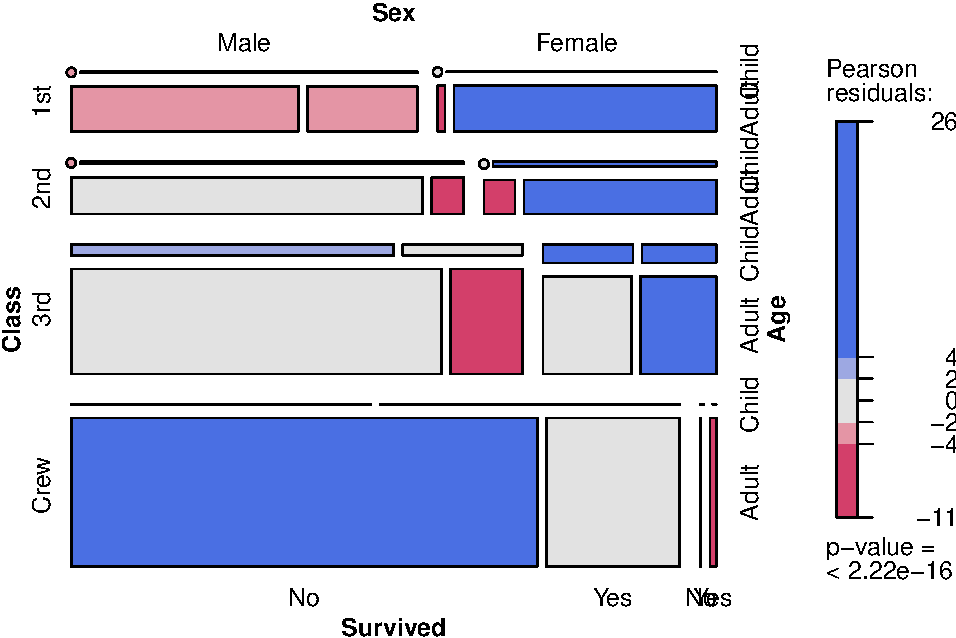
\includegraphics{AEProject_files/figure-latex/unnamed-chunk-1-1.pdf}

\hypertarget{preprocessing}{%
\subsection{3.2.Preprocessing}\label{preprocessing}}

As previously mentioned we started our data preprocessing with merging
respectively datasets to get complete data for further transformations.

\begin{verbatim}
##   PassengerId Survived Pclass
## 1           1        0      3
## 2           2        1      1
## 3           3        1      3
## 4           4        1      1
## 5           5        0      3
## 6           6        0      3
##                                                  Name    Sex Age SibSp Parch
## 1                             Braund, Mr. Owen Harris   male  22     1     0
## 2 Cumings, Mrs. John Bradley (Florence Briggs Thayer) female  38     1     0
## 3                              Heikkinen, Miss. Laina female  26     0     0
## 4        Futrelle, Mrs. Jacques Heath (Lily May Peel) female  35     1     0
## 5                            Allen, Mr. William Henry   male  35     0     0
## 6                                    Moran, Mr. James   male  NA     0     0
##             Ticket    Fare Cabin Embarked
## 1        A/5 21171  7.2500              S
## 2         PC 17599 71.2833   C85        C
## 3 STON/O2. 3101282  7.9250              S
## 4           113803 53.1000  C123        S
## 5           373450  8.0500              S
## 6           330877  8.4583              Q
\end{verbatim}

\begin{verbatim}
##   PassengerId      Survived          Pclass          Name          
##  Min.   :   1   Min.   :0.0000   Min.   :1.000   Length:1309       
##  1st Qu.: 328   1st Qu.:0.0000   1st Qu.:2.000   Class :character  
##  Median : 655   Median :0.0000   Median :3.000   Mode  :character  
##  Mean   : 655   Mean   :0.3774   Mean   :2.295                     
##  3rd Qu.: 982   3rd Qu.:1.0000   3rd Qu.:3.000                     
##  Max.   :1309   Max.   :1.0000   Max.   :3.000                     
##                                                                    
##      Sex                 Age            SibSp            Parch      
##  Length:1309        Min.   : 0.17   Min.   :0.0000   Min.   :0.000  
##  Class :character   1st Qu.:21.00   1st Qu.:0.0000   1st Qu.:0.000  
##  Mode  :character   Median :28.00   Median :0.0000   Median :0.000  
##                     Mean   :29.88   Mean   :0.4989   Mean   :0.385  
##                     3rd Qu.:39.00   3rd Qu.:1.0000   3rd Qu.:0.000  
##                     Max.   :80.00   Max.   :8.0000   Max.   :9.000  
##                     NA's   :263                                     
##     Ticket               Fare            Cabin             Embarked        
##  Length:1309        Min.   :  0.000   Length:1309        Length:1309       
##  Class :character   1st Qu.:  7.896   Class :character   Class :character  
##  Mode  :character   Median : 14.454   Mode  :character   Mode  :character  
##                     Mean   : 33.295                                        
##                     3rd Qu.: 31.275                                        
##                     Max.   :512.329                                        
##                     NA's   :1
\end{verbatim}

Since the data can have missing fields, incomplete fields, or fields
containing hidden or useless information, a crucial step is to remove
them in order not to complicate the further analysis. Variables
\texttt{Fare}, \texttt{Age} and \texttt{Embarked} will not be used, so
we decided to remove them. Especially embarked variable will not be used
as is not individual specific.

Our second hypothesis has to verify whether having a family on board has
increased the chance of passenger to survive, therefore a new variable
\texttt{Family} has been created as a sum of already existing variables
\texttt{SibSp} - number of siblings and spouses of the passenger aboard
and \texttt{Parch}- number of parents and children of the passenger
aboard.

\begin{verbatim}
##   PassengerId Survived Pclass
## 1           1       No      3
## 2           2      Yes      1
## 3           3      Yes      3
## 4           4      Yes      1
## 5           5       No      3
## 7           7       No      1
##                                                  Name    Sex Age SibSp Parch
## 1                             Braund, Mr. Owen Harris   male  22     1     0
## 2 Cumings, Mrs. John Bradley (Florence Briggs Thayer) female  38     1     0
## 3                              Heikkinen, Miss. Laina female  26     0     0
## 4        Futrelle, Mrs. Jacques Heath (Lily May Peel) female  35     1     0
## 5                            Allen, Mr. William Henry   male  35     0     0
## 7                             McCarthy, Mr. Timothy J   male  54     0     0
##             Ticket    Fare Cabin Embarked Family
## 1        A/5 21171  7.2500              S      1
## 2         PC 17599 71.2833   C85        C      1
## 3 STON/O2. 3101282  7.9250              S      0
## 4           113803 53.1000  C123        S      1
## 5           373450  8.0500              S      0
## 7            17463 51.8625   E46        S      0
\end{verbatim}

\hypertarget{application-of-econometric-models}{%
\section{4. Application of Econometric
Models}\label{application-of-econometric-models}}

\hypertarget{exploring-and-test-multinom-models}{%
\section{Exploring and Test Multinom
Models}\label{exploring-and-test-multinom-models}}

Generating 4 models using multinom function.

Formulas for models,

model1 \textless- Survived \textasciitilde{} Sex + Pclass + Age + Family
+ Fare + Farepp + Embarked + SibSp + Parch model2 \textless- Survived
\textasciitilde{} Sex + Pclass + Age + Family + Embarked + SibSp + Parch
model3 \textless- Survived \textasciitilde{} Sex + Pclass + Age + Family
+ SibSp + Parch model4 \textless- Survived \textasciitilde{} Sex +
Pclass + Age + Family -

\begin{verbatim}
## # weights:  13 (12 variable)
## initial  value 722.952509 
## iter  10 value 418.303559
## iter  20 value 391.968038
## iter  20 value 391.968037
## iter  20 value 391.968037
## final  value 391.968037 
## converged
\end{verbatim}

\begin{verbatim}
## # weights:  11 (10 variable)
## initial  value 722.952509 
## iter  10 value 429.162839
## final  value 392.309873 
## converged
\end{verbatim}

\begin{verbatim}
## # weights:  9 (8 variable)
## initial  value 722.952509 
## iter  10 value 392.953976
## final  value 392.735365 
## converged
\end{verbatim}

\begin{verbatim}
## # weights:  7 (6 variable)
## initial  value 722.952509 
## iter  10 value 393.518417
## final  value 393.495630 
## converged
\end{verbatim}

Performing statistical significance

\begin{verbatim}
## 
## ===============================================================================================
## (Intercept) Sexmale Pclass2 Pclass3 SibSp  Parch Family EmbarkedQ EmbarkedS Fare   Age   Farepp
## -----------------------------------------------------------------------------------------------
## 9.180       -17.459 -3.826  -6.720  -1.797 0.357 -2.499  -0.554    -0.711   0.209 -4.809 0.271 
## -----------------------------------------------------------------------------------------------
## 
## ==================================================================================
## (Intercept) Sexmale Pclass2 Pclass3 SibSp  Parch Family EmbarkedQ EmbarkedS  Age  
## ----------------------------------------------------------------------------------
## 10.603      -17.535 -4.497  -8.092  -1.831 0.431 -2.936  -0.623    -0.878   -4.859
## ----------------------------------------------------------------------------------
## 
## ==============================================================
## (Intercept) Sexmale Pclass2 Pclass3 SibSp  Parch Family  Age  
## --------------------------------------------------------------
## 10.747      -17.700 -5.084  -8.879  -1.888 0.475 -2.978 -4.964
## --------------------------------------------------------------
## 
## =================================================
## (Intercept) Sexmale Pclass2 Pclass3 Family  Age  
## -------------------------------------------------
## 10.718      -17.817 -5.045  -8.845  -2.934 -4.870
## -------------------------------------------------
\end{verbatim}

Performing 2-tailed z test

\begin{verbatim}
## 
## ===============================================================================================
## (Intercept) Sexmale Pclass2 Pclass3 SibSp Parch Family EmbarkedQ EmbarkedS Fare    Age   Farepp
## -----------------------------------------------------------------------------------------------
## 0              0    0.0001     0    0.072 0.721 0.012    0.580     0.477   0.834 0.00000 0.786 
## -----------------------------------------------------------------------------------------------
## 
## ==================================================================================
## (Intercept) Sexmale Pclass2 Pclass3 SibSp Parch Family EmbarkedQ EmbarkedS   Age  
## ----------------------------------------------------------------------------------
## 0              0    0.00001    0    0.067 0.667 0.003    0.533     0.380   0.00000
## ----------------------------------------------------------------------------------
## 
## ==============================================================
## (Intercept) Sexmale Pclass2 Pclass3 SibSp Parch Family   Age  
## --------------------------------------------------------------
## 0              0    0.00000    0    0.059 0.635 0.003  0.00000
## --------------------------------------------------------------
## 
## ==================================================
## (Intercept) Sexmale Pclass2 Pclass3 Family   Age  
## --------------------------------------------------
## 0              0    0.00000    0    0.003  0.00000
## --------------------------------------------------
\end{verbatim}

\begin{verbatim}
## 
## =========================================================
##                             Dependent variable:          
##                   ---------------------------------------
##                                  Survived                
##                      (1)       (2)       (3)       (4)   
## ---------------------------------------------------------
## Sexmale           -3.686*** -3.693*** -3.691*** -3.703***
##                    (0.211)   (0.211)   (0.209)   (0.208) 
##                                                          
## Pclass2           -1.150*** -1.241*** -1.322*** -1.306***
##                    (0.301)   (0.276)   (0.260)   (0.259) 
##                                                          
## Pclass3           -2.089*** -2.202*** -2.285*** -2.271***
##                    (0.311)   (0.272)   (0.257)   (0.257) 
##                                                          
## SibSp              -0.172*   -0.175*   -0.179*           
##                    (0.095)   (0.095)   (0.095)           
##                                                          
## Parch               0.034     0.040     0.044            
##                    (0.095)   (0.092)   (0.092)           
##                                                          
## Family            -0.138**  -0.135*** -0.135*** -0.199***
##                    (0.055)   (0.046)   (0.045)   (0.068) 
##                                                          
## EmbarkedQ          -0.275    -0.308                      
##                    (0.496)   (0.494)                     
##                                                          
## EmbarkedS          -0.175    -0.212                      
##                    (0.247)   (0.242)                     
##                                                          
## Fare                0.001                                
##                    (0.004)                               
##                                                          
## Age               -0.036*** -0.036*** -0.037*** -0.036***
##                    (0.007)   (0.007)   (0.007)   (0.007) 
##                                                          
## Farepp              0.001                                
##                    (0.005)                               
##                                                          
## Constant          4.371***  4.544***  4.447***  4.411*** 
##                    (0.476)   (0.429)   (0.414)   (0.412) 
##                                                          
## ---------------------------------------------------------
## Akaike Inf. Crit.  805.936   802.620   799.471   798.991 
## =========================================================
## Note:                         *p<0.1; **p<0.05; ***p<0.01
\end{verbatim}

\hypertarget{exploring-mlogit-data-and-model}{%
\section{Exploring MLogit Data and
Model}\label{exploring-mlogit-data-and-model}}

Generating data in mlogit.data format

\begin{verbatim}
## ~~~~~~~
##  first 10 observations out of 2086 
## ~~~~~~~
##       Sex Pclass SibSp Parch Family Embarked Survived    Fare Age   Farepp chid
## 1    male      3     1     0      1        S     TRUE  7.2500  22  3.62500    1
## 2    male      3     1     0      1        S    FALSE  7.2500  22  3.62500    1
## 3  female      1     1     0      1        C    FALSE 71.2833  38 35.64165    2
## 4  female      1     1     0      1        C     TRUE 71.2833  38 35.64165    2
## 5  female      3     0     0      0        S    FALSE  7.9250  26  7.92500    3
## 6  female      3     0     0      0        S     TRUE  7.9250  26  7.92500    3
## 7  female      1     1     0      1        S    FALSE 53.1000  35 26.55000    4
## 8  female      1     1     0      1        S     TRUE 53.1000  35 26.55000    4
## 9    male      3     0     0      0        S     TRUE  8.0500  35  8.05000    5
## 10   male      3     0     0      0        S    FALSE  8.0500  35  8.05000    5
##    alt   idx
## 1   No  1:No
## 2  Yes 1:Yes
## 3   No  2:No
## 4  Yes 2:Yes
## 5   No  3:No
## 6  Yes 3:Yes
## 7   No  4:No
## 8  Yes 4:Yes
## 9   No  5:No
## 10 Yes 5:Yes
## 
## ~~~ indexes ~~~~
##    chid alt
## 1     1  No
## 2     1 Yes
## 3     2  No
## 4     2 Yes
## 5     3  No
## 6     3 Yes
## 7     4  No
## 8     4 Yes
## 9     5  No
## 10    5 Yes
## indexes:  1, 2
\end{verbatim}

Running the model on mlogit data

\begin{verbatim}
## 
## Call:
## mlogit(formula = Survived ~ 0 | Sex + Family + Pclass + Age,     data = mldf, method = "nr")
## 
## Coefficients:
## (Intercept):Yes      Sexmale:Yes       Family:Yes      Pclass2:Yes  
##        4.411308        -3.703381        -0.199020        -1.306308  
##     Pclass3:Yes          Age:Yes  
##       -2.271218        -0.035976
\end{verbatim}

Summary of the mlogit model

\begin{verbatim}
## 
## Call:
## mlogit(formula = Survived ~ 0 | Sex + Family + Pclass + Age, 
##     data = mldf, method = "nr")
## 
## Frequencies of alternatives:choice
##      No     Yes 
## 0.60211 0.39789 
## 
## nr method
## 6 iterations, 0h:0m:0s 
## g'(-H)^-1g = 1.91E-06 
## successive function values within tolerance limits 
## 
## Coefficients :
##                   Estimate Std. Error  z-value  Pr(>|z|)    
## (Intercept):Yes  4.4113075  0.4115900  10.7177 < 2.2e-16 ***
## Sexmale:Yes     -3.7033811  0.2078565 -17.8170 < 2.2e-16 ***
## Family:Yes      -0.1990198  0.0678444  -2.9335  0.003352 ** 
## Pclass2:Yes     -1.3063077  0.2589408  -5.0448  4.54e-07 ***
## Pclass3:Yes     -2.2712179  0.2567849  -8.8448 < 2.2e-16 ***
## Age:Yes         -0.0359755  0.0073881  -4.8694  1.12e-06 ***
## ---
## Signif. codes:  0 '***' 0.001 '**' 0.01 '*' 0.05 '.' 0.1 ' ' 1
## 
## Log-Likelihood: -393.5
## McFadden R^2:  0.4387 
## Likelihood ratio test : chisq = 615.11 (p.value = < 2.22e-16)
\end{verbatim}

\hypertarget{results-findings}{%
\section{5. Results \& Findings}\label{results-findings}}

\hypertarget{part-a}{%
\subsection{Part A}\label{part-a}}

We compare the restricted model to the unrestricted model to obtain the
joint significance test. Number of restrictions are 4. We compare the
restricted model to the constant model using likelihood ratio test.

p-value = 2.2 e-16 and LR test = 615.11

Null hypothesis: Pclass = 0, Sex = 0, Family = 0 and Age = 0

The p-value is lower than the significance level of 0.05. Therefore, we
have to reject the null hypothesis which states parameters are jointly
insignificant. \textbf{The parameters are jointly significant. }

\begin{verbatim}
## # weights:  7 (6 variable)
## initial  value 722.952509 
## iter  10 value 393.518417
## final  value 393.495630 
## converged
\end{verbatim}

\begin{verbatim}
## # weights:  2 (1 variable)
## initial  value 722.952509 
## final  value 701.049473 
## converged
\end{verbatim}

\begin{verbatim}
## Likelihood ratio test
## 
## Model 1: Survived ~ Pclass + Sex + Family + Age
## Model 2: Survived ~ 1
##   #Df  LogLik Df  Chisq Pr(>Chisq)    
## 1   6 -393.50                         
## 2   1 -701.05 -5 615.11  < 2.2e-16 ***
## ---
## Signif. codes:  0 '***' 0.001 '**' 0.01 '*' 0.05 '.' 0.1 ' ' 1
\end{verbatim}

\hypertarget{part-b}{%
\subsection{Part B}\label{part-b}}

The model is created with non linear relation (square of Fare) and
interactions between Age:Pclass \& Sex:Pclass. The Fare and Fare\^{}2
both have a p-value \textless{} 0.05. Similarly, for Pclass2:Age,
Sexmale:Pclass2 and Sexmale:Pclass3 have p-value \textless{} 0.05. This
means, we reject the null hypothesis. The parameters add meaningful
addition to model. Pclass:Age interaction is insignificant.

\begin{verbatim}
## # weights:  12 (11 variable)
## initial  value 722.952509 
## iter  10 value 398.759983
## iter  20 value 373.133076
## final  value 373.132688 
## converged
\end{verbatim}

\begin{verbatim}
## 
## =============================================
##                       Dependent variable:    
##                   ---------------------------
##                            Survived          
## ---------------------------------------------
## Fare                       -0.015***         
##                             (0.004)          
##                                              
## Fare2                     0.00004***         
##                            (0.00001)         
##                                              
## Sexmale                    -5.104***         
##                            (0.0001)          
##                                              
## Pclass2                    0.357***          
##                            (0.0003)          
##                                              
## Pclass3                    -4.525***         
##                            (0.0003)          
##                                              
## Age                        -0.029***         
##                             (0.006)          
##                                              
## Pclass2:Age                -0.064***         
##                             (0.009)          
##                                              
## Pclass3:Age                  0.003           
##                             (0.007)          
##                                              
## Sexmale:Pclass2            -0.799***         
##                            (0.0002)          
##                                              
## Sexmale:Pclass3            2.453***          
##                            (0.0001)          
##                                              
## Constant                   5.900***          
##                            (0.0002)          
##                                              
## ---------------------------------------------
## Akaike Inf. Crit.           768.265          
## =============================================
## Note:             *p<0.1; **p<0.05; ***p<0.01
\end{verbatim}

\hypertarget{part-c}{%
\subsection{Part C}\label{part-c}}

Marginal effects are used to quantify the incremental risk associated
with each factor.We start by creating a vector z which contains average
characterstics.

The effect of Fare on Survival for each increment is by 0.3\%. More the
fare, more chances of survival.

\begin{verbatim}
## 
## ============
## No      Yes 
## ------------
## -0.003 0.003
## ------------
\end{verbatim}

The effect of Family size on Survival for each increment in Family
members is by -0.7\%. More the family, lesser the chances of survival.

\begin{verbatim}
## 
## ============
## No     Yes  
## ------------
## 0.007 -0.007
## ------------
\end{verbatim}

The effect of Age on Survival for each increment in Age is by -0.4\%.
Older the person, lesser the chances of survival.

\begin{verbatim}
## 
## ============
## No     Yes  
## ------------
## 0.004 -0.004
## ------------
\end{verbatim}

\hypertarget{part-d}{%
\subsection{Part D}\label{part-d}}

The final model is (3) in the table which can be represented by the
formula:

log(P(Survived=Yes)/P(Survived=No)) = 4.411 + (-3.703 * Sexmale) +
(-1.306 * Pclass2) + (-2.271 * Pclass3) + (-0.199 * Family) + (-0.036 *
Age)

\begin{verbatim}
## # weights:  9 (8 variable)
## initial  value 722.952509 
## iter  10 value 378.827124
## final  value 378.275558 
## converged
\end{verbatim}

\begin{verbatim}
## 
## ===============================================
##                        Dependent variable:     
##                   -----------------------------
##                             Survived           
##                      (1)       (2)       (3)   
## -----------------------------------------------
## Sexmale           -3.686*** -4.927*** -3.703***
##                    (0.211)   (0.622)   (0.208) 
##                                                
## Pclass2           -1.150***  -1.382*  -1.306***
##                    (0.301)   (0.731)   (0.259) 
##                                                
## Pclass3           -2.089*** -3.834*** -2.271***
##                    (0.311)   (0.635)   (0.257) 
##                                                
## SibSp              -0.172*                     
##                    (0.095)                     
##                                                
## Parch               0.034                      
##                    (0.095)                     
##                                                
## Family            -0.138**  -0.189*** -0.199***
##                    (0.055)   (0.067)   (0.068) 
##                                                
## EmbarkedQ          -0.275                      
##                    (0.496)                     
##                                                
## EmbarkedS          -0.175                      
##                    (0.247)                     
##                                                
## Fare                0.001                      
##                    (0.004)                     
##                                                
## Age               -0.036*** -0.040*** -0.036***
##                    (0.007)   (0.008)   (0.007) 
##                                                
## Farepp              0.001                      
##                    (0.005)                     
##                                                
## Sexmale:Pclass2              -0.322            
##                              (0.798)           
##                                                
## Sexmale:Pclass3             2.166***           
##                              (0.667)           
##                                                
## Constant          4.371***  5.606***  4.411*** 
##                    (0.476)   (0.703)   (0.412) 
##                                                
## -----------------------------------------------
## Akaike Inf. Crit.  805.936   772.551   798.991 
## ===============================================
## Note:               *p<0.1; **p<0.05; ***p<0.01
\end{verbatim}

\hypertarget{part-e}{%
\subsection{Part E}\label{part-e}}

The linktest is used to check the appropriate form of the model. The
motivation behind the link test is the idea that if a regression is
specified appropriately you should not be able to find additional
independent variables.

The condition for linktest is to have yhat as significant and yhat\^{}2
as insgnificant. (Ho: The model has appropriate form)

In the below model, we have yhat as significant and yhat2 as
insignificant. Therefore, we fail to reject the null hypothesis. The
model has an an appropriate form.

\begin{verbatim}
## # weights:  9 (8 variable)
## initial  value 722.952509 
## iter  10 value 378.827124
## final  value 378.275558 
## converged
\end{verbatim}

\begin{verbatim}
## # weights:  4 (3 variable)
## initial  value 722.952509 
## iter  10 value 378.950785
## final  value 377.982713 
## converged
## Call:
## multinom(formula = y ~ yhat + yhat2)
## 
## Coefficients:
##                  Values  Std. Err.
## (Intercept)  0.06860774 0.13547628
## yhat         1.00262896 0.05820039
## yhat2       -0.02252481 0.02900746
## 
## Residual Deviance: 755.9654 
## AIC: 761.9654
\end{verbatim}

\begin{verbatim}
## 
## =============================================
##                       Dependent variable:    
##                   ---------------------------
##                                y             
## ---------------------------------------------
## yhat                       1.003***          
##                             (0.058)          
##                                              
## yhat2                       -0.023           
##                             (0.029)          
##                                              
## Constant                     0.069           
##                             (0.135)          
##                                              
## ---------------------------------------------
## Akaike Inf. Crit.           761.965          
## =============================================
## Note:             *p<0.1; **p<0.05; ***p<0.01
\end{verbatim}

\hypertarget{hypothesis-testing}{%
\subsection{Hypothesis Testing}\label{hypothesis-testing}}

\textbf{Hypothesis 1}

H0: Having a seat in higher class insignificant to survive.

H1: Having a seat in higher class is significant to survive.

\textbf{Result 1}

The parameters Pclass2 and Pclass3 are significant as their p-value is
\textless{} 0.05. Having a seat in class 2 and class 3 is significant to
survival but as the coefficient is negative it decreases the probability
of survival.The rate of survival is class 2 is more than in class 3. The
rate of survival in class 1 is the most as pclass 2 = 0 and pclass 3 =
0.

Therefore, we reject the null hypothesis. Having a seat in higher class
indeed increases the chance of passenger to survive.

\textbf{Hypothesis 2}

H0: Paying a higher fare/having a family member on board is
insignificant to survive.

H1: Paying a higher fare/having a family member on board is significant
survival.

\textbf{Result 2}

Fare is insignificant as the p-value is greater than 0.05. We fail to
reject the null hypothesis. Paying a higher fare is insignificant to
survival.

However, having a family member on board is significant as the p-value
is less than 0.05. We reject the null hypothesis. Having a family member
on board is significant for survival. As the coefficient is negative, it
is in fact reducing the probability to survive significantly.

\begin{verbatim}
## # weights:  8 (7 variable)
## initial  value 722.952509 
## iter  10 value 393.222368
## final  value 392.965611 
## converged
\end{verbatim}

\begin{verbatim}
## 
## =============================================
##                       Dependent variable:    
##                   ---------------------------
##                            Survived          
## ---------------------------------------------
## Pclass2                    -1.173***         
##                             (0.290)          
##                                              
## Pclass3                    -2.109***         
##                             (0.302)          
##                                              
## Age                        -0.036***         
##                             (0.007)          
##                                              
## Sexmale                    -3.697***         
##                             (0.208)          
##                                              
## Family                     -0.219***         
##                             (0.071)          
##                                              
## Fare                         0.002           
##                             (0.002)          
##                                              
## Constant                   4.232***          
##                             (0.447)          
##                                              
## ---------------------------------------------
## Akaike Inf. Crit.           799.931          
## =============================================
## Note:             *p<0.1; **p<0.05; ***p<0.01
\end{verbatim}

\hypertarget{conclusions}{%
\section{Conclusions}\label{conclusions}}

In our analysis, we concluded that an econometric model can be useful in
predicting what features increases survival rate during sinking of the
Titanic in 1912. As we know from literature one of the reasons that the
shipwreck lead to such loss of life is that were not enough lifeboats
for the passengers and crew. Although there was some element of luck
involved in surviving the sinking, some groups of people were more
likely to survive than others, like younger passengers, the upper-class
and those who had no family members on board which we confirmed with the
results of the Multinomial Logit Model.

\hypertarget{bibliography}{%
\section{Bibliography}\label{bibliography}}

\begin{enumerate}
\def\labelenumi{\arabic{enumi}.}
\item
  Whitley M., ``Using statistical learning to predict survival of
  passengers on the RMS Titanic'' K-State Research Exchange, (1), 2015,
  pp.~32
\item
  Kshirsagar V., Phalke N., ``Titanic Survival Analysis using Logistic
  Regression'' International Research Journal of Engineering and
  Technology (IRJET), (2), 2019, pp.~90︎
\item
  Donges N., ``Predicting the Survival of Titanic Passengers''
  towardsdatascience.com, (3), 2018
\end{enumerate}

\end{document}
